\documentclass{article}
\usepackage{include/nips13submit_e,times}
%%%%%%%%%%%%%%%%%%%%%%%%%%%%%%%%%%%%%%%%%%%%%%%%%%%%%%%%%%%
%%%% EDITING HELPER FUNCTIONS  %%%%%%%%%%%%%%%%%%%%%%%%%%%
%%%%%%%%%%%%%%%%%%%%%%%%%%%%%%%%%%%%%%%%%%%%%%%%%%%%%%%%%%

%% NA: needs attention (rough writing whose correctness needs to be verified)
%% TBD: instructions for how to fix a gap ("Describe the propagation by ...")
%% PROBLEM: bug or missing crucial bit 

%% use \fXXX versions of these macros to put additional explanation into a footnote.  
%% The idea is that we don't want to interrupt the flow of the paper or make it 
%% impossible to read because there are a bunch of comments.

%% NA's (and TBDs, those less crucially) should be written so 
%% that they flow with the text.

\definecolor{WowColor}{rgb}{.75,0,.75}
\definecolor{SubtleColor}{rgb}{0,0,.50}

% inline
\newcommand{\NA}[1]{\textcolor{SubtleColor}{ {\tiny \bf ($\star$)} #1}}
\newcommand{\LATER}[1]{\textcolor{SubtleColor}{ {\tiny \bf ($\dagger$)} #1}}
\newcommand{\TBD}[1]{\textcolor{SubtleColor}{ {\tiny \bf (!)} #1}}
\newcommand{\PROBLEM}[1]{\textcolor{WowColor}{ {\bf (!!)} {\bf #1}}}

% as margin notes

\newcounter{margincounter}
\newcommand{\displaycounter}{{\arabic{margincounter}}}
\newcommand{\incdisplaycounter}{{\stepcounter{margincounter}\arabic{margincounter}}}

\newcommand{\fTBD}[1]{\textcolor{SubtleColor}{$\,^{(\incdisplaycounter)}$}\marginpar{\tiny\textcolor{SubtleColor}{ {\tiny $(\displaycounter)$} #1}}}

\newcommand{\fPROBLEM}[1]{\textcolor{WowColor}{$\,^{((\incdisplaycounter))}$}\marginpar{\tiny\textcolor{WowColor}{ {\bf $\mathbf{((\displaycounter))}$} {\bf #1}}}}

\newcommand{\fLATER}[1]{\textcolor{SubtleColor}{$\,^{(\incdisplaycounter\dagger)}$}\marginpar{\tiny\textcolor{SubtleColor}{ {\tiny $(\displaycounter\dagger)$} #1}}}

\usepackage{include/preamble}
\usepackage{natbib}

\title{Non-degenerate Priors for Arbitrarily Deep Networks}


\author{
David Duvenaud \\
University of Cambridge \\
\texttt{dkd23@cam.ac.uk} \\
\And
Oren Rippel \\
Harvard University \\
\texttt{rippel@math.mit.edu} \\
\And
Ryan Adams \\
Harvard University \\
\texttt{rpa@seas.harvard.edu} \\
}

% Custom notation
\newcommand{\fdeep}{f^{1:L}}
\newcommand{\flast}{f^{L}}
\newcommand{\Jx}{J_{\vx \rightarrow \vy}}
\newcommand{\Jxx}{J_{\vx \rightarrow \vy}(\vx)}
\newcommand{\Jy}{J_{\vy \rightarrow \vx}}
\newcommand{\Jyy}{J_{\vy \rightarrow \vx}(\vy)}
\newcommand{\detJyy}{ \left| J_{\vy \rightarrow \vx}(\vy) \right|}


% The \author macro works with any number of authors. There are two commands
% used to separate the names and addresses of multiple authors: \And and \AND.
%
% Using \And between authors leaves it to \LaTeX{} to determine where to break
% the lines. Using \AND forces a linebreak at that point. So, if \LaTeX{}
% puts 3 of 4 authors names on the first line, and the last on the second
% line, try using \AND instead of \And before the third author name.

\newcommand{\fix}{\marginpar{FIX}}
\newcommand{\new}{\marginpar{NEW}}

%\nipsfinalcopy % Uncomment for camera-ready version

\begin{document}


\maketitle

\begin{abstract}
%We first demonstrate a pathology of typical deep architectures: as the number of layers increase, latent representations 
A good latent representation captures all the relevant degrees of freedom of the manifold on which the data live.  We show, for typical deep architectures, that as the number of layers increase, the representational capacity of the model tends to capture fewer degrees of freedom.  In the limit, deep representations only retain a single degree of freedom locally.  In addition, gradient-based learning becomes intractable.  We propose several solutions to address these pathologies.
\end{abstract}

\section{Introduction}

Deep networks have become an important tool for machine learning [cite].  However, training these models are difficult, Many arguments have been made for the need for deep architectures [cite Bengio].  However, it is hard to know what effect the deepness of an architecture has.  Also, the weights don't necessarily move that much from their initialization.

\subsection{Desirable properties of latent representations}

\cite{rifai2011higher} make the point that a good latent representation is one that remains invariant when moving in directions orthogonal to the manifold that the data lie on.  Conversely, a good latent representation must also change in directions tangential to the data manifold - otherwise we are losing information about the data.


\section{The Jacobian of Deep GPs}

\paragraph{Deep Gaussian Processes}
We introduce a generative non-parametric model to address this problem.  Our approach is based on the GP-LVM ~\cite{lawrence2004gaussian,salzmann2008local,lawrence2009non}, a flexible nonparametric density model.  Deep Gaussian processes \cite{damianou2012deep}.


\paragraph{The derivatives of a function drawn from a \gp{} prior with a product kernel are \iid Normal}

Because differentiation is a linear operator, the derivatives of a function drawn from a \gp{} prior are also jointly Gaussian distributed, with covariance between derivatives w.r.t. different dimensions of $\vx$ given by:
%
\begin{align}
\cov \left( \frac{\partial f(\vx)}{\partial x_{d_1}}, \frac{\partial f(\vx)}{\partial x_{d_2}} \right) =
\frac{\partial^2 k(\vx, \vx'))}{\partial x_{d_1} \partial x_{d_2}'} \bigg|_{\vx=\vx'}
\end{align}
%
\cite{Solak03derivativeobservations}

If our kernel is a product over individual dimensions $k(\vx, \vx') = \prod_d^D k_d(x_d, x_d')$, as in the case of the isotropic squared-exp kernel, then the diagonal covariances are given by $\frac{\sigma_o^2}{\ell^2}$, and the off-diagonal entries are zero.  This means that elements are independent and identically distributed.

\paragraph{The elements of the Jacobian of a \gp{} with an isotropic SE kernel are \iid Gaussians}

The Jacobian of the $\ell$\asdf function is:
%
\begin{align}
\Jx^\ell(\vx) =\begin{bmatrix} \dfrac{\partial f^\ell_1 (\vx) }{\partial x_1} & \cdots & \dfrac{\partial f^\ell_1 (\vx)}{\partial x_D} \\ \vdots & \ddots & \vdots \\ \dfrac{\partial f^\ell_D (\vx)}{\partial x_1} & \cdots & \dfrac{\partial f^\ell_D (\vx)}{\partial x_D}  \end{bmatrix}
\end{align}
%
Because we've assumed that the \gp{} on each output dimension $f_d(\vx) \sim \GP$ is independent, it follows that for a given $\vx$, each row of $\Jxx$ is independent.
Above, we showed that the elements of each row are independent.
This means that each entry in the Jacobian of a \gp{}-distributed transformation is \iid Normal.

%We also have that if $\vx = f(\vy)$, then $\Jy\inv(\vy) = \Jxx$.

\paragraph{The Jacobian of a deep \gp{} is a product of random normal matrices}
By the multivariate chain rule, the derivative (Jacobian) of any compositions of functions is simply the product of the Jacobians of each function.  
%
and the Jacobian of the composed (deep) function is:
%
\begin{align}
J^{1:L}(x) 
% = \frac{\partial \fdeep(x) }{\partial x} 
%= \frac{\partial f^1(x) }{\partial x} \frac{\partial f^2(x) }{\partial f^1(x)} \cdots \frac{\partial f^L(x) }{\partial f^{L-1}(x)}
= \prod_{\ell = 1}^{L} J^L (x)
\end{align}

Combining these results, we can analyze the representational properties of a deep Gaussian process by simply examining the properties of products of i.i.d. Gaussian matrices.

We follow \cite{rifai2011contractive} in characterizing the representational properties of a function by the singular value spectrum of the Jacobian.  Figure \ref{fig:deep_spectrum} shows the spectrum for deep GPs of different depths.

\begin{figure}
\centering
\begin{tabular}{ccc}
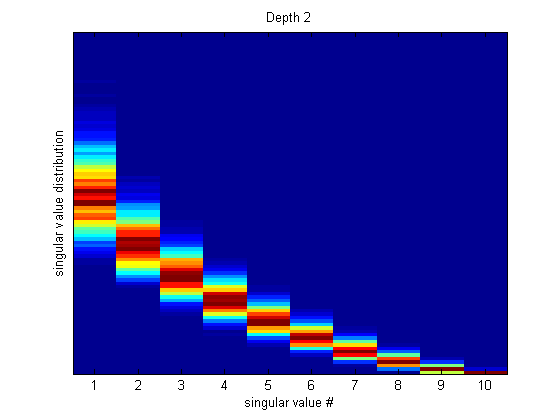
\includegraphics[width=0.3\columnwidth]{figures/spectrum/svd_specturm_depth_2} &
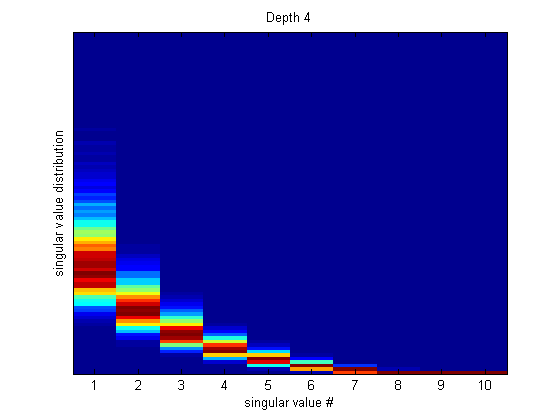
\includegraphics[width=0.3\columnwidth]{figures/spectrum/svd_specturm_depth_4} &
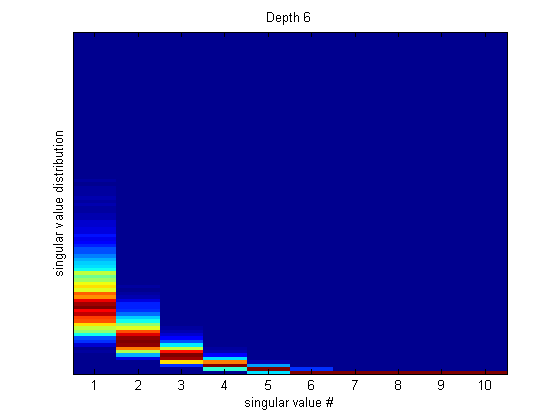
\includegraphics[width=0.3\columnwidth]{figures/spectrum/svd_specturm_depth_6} \\
2 layers & 4 layers & 6 layers
\end{tabular}
\caption{Singular value spectrum of the Jacobian of a deep GP.  As the net gets deeper, the largest singular value dominates.  This implies that there is only one effective degree of freedom in representation being computed.}
\label{fig:deep_spectrum}
\end{figure}



\begin{figure}
\centering
\begin{tabular}{ccc}
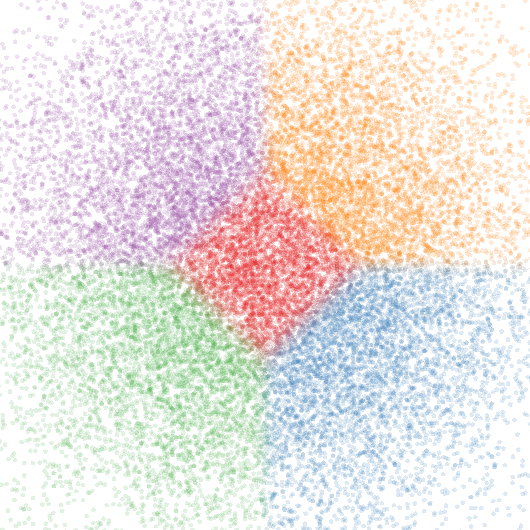
\includegraphics[width=0.3\columnwidth]{figures/deep_draws/deep_gp_sample_layer_1} &
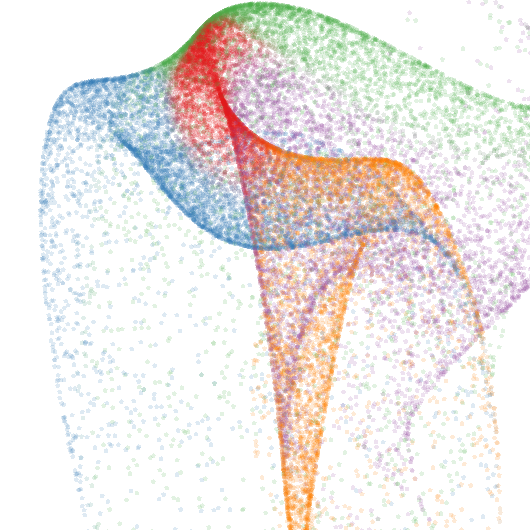
\includegraphics[width=0.3\columnwidth]{figures/deep_draws/deep_gp_sample_layer_2} &
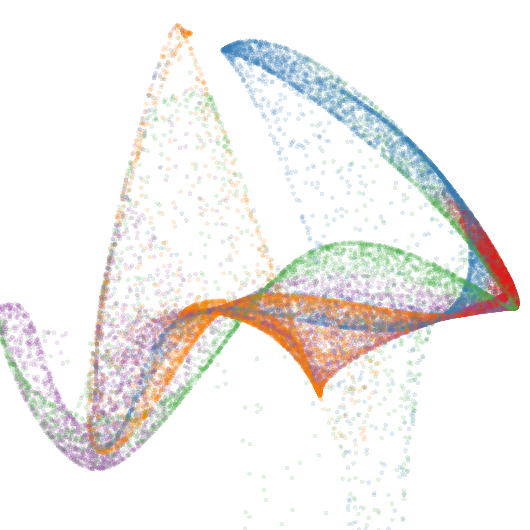
\includegraphics[width=0.3\columnwidth]{figures/deep_draws/deep_gp_sample_layer_3} \\
$p(\vx)$ & $p(f_1(\vx))$ & $p(f_2(f_1(\vx)))$ \\ \\
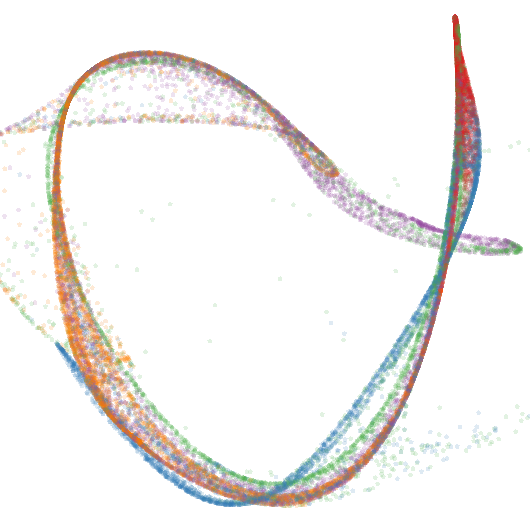
\includegraphics[width=0.3\columnwidth]{figures/deep_draws/deep_gp_sample_layer_4} &
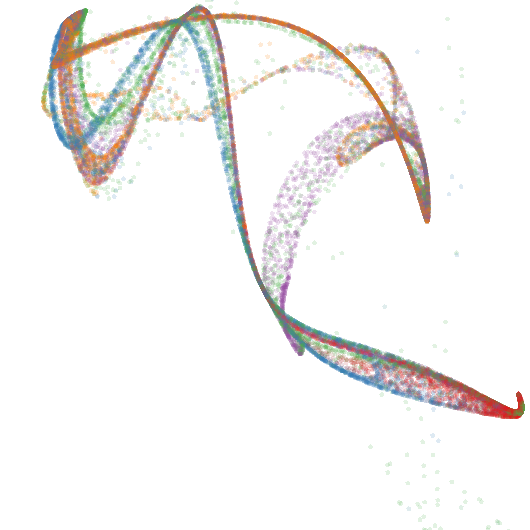
\includegraphics[width=0.3\columnwidth]{figures/deep_draws/deep_gp_sample_layer_5} &
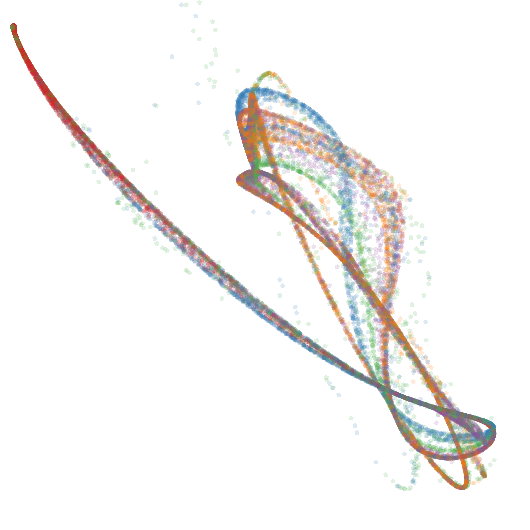
\includegraphics[width=0.3\columnwidth]{figures/deep_draws/deep_gp_sample_layer_6} \\
$p(f_3(f_2(f_1(\vx))))$ & $p(f_4(f_3(f_2(f_1(\vx)))))$ & $p(f_5(f_4(f_3(f_2(f_1(\vx)))))$
\end{tabular}
\caption{Draws from a deep GP.  A distribution is warped by successive functions drawn from a \gp{} prior.  As the number of layers increases, the density exhibits a sort of filamentation.}
\label{fig:filamentation}
\end{figure}


\newcommand{\mappic}[1]{\includegraphics[width=0.3\columnwidth]{figures/map/latent_coord_map_layer_#1}} 

\begin{figure}
\centering
\begin{tabular}{ccc}
\mappic{0} & \mappic{1} & \mappic{2} \\
Identity Map: $\vy = \vx$ & 1 Layer: $\vy = f_1(\vx)$ & 2 Layers: $\vy = f_1(f_2(\vx))$ \\
\mappic{4} & \mappic{10} & \mappic{40} \\
4 Layers & 10 Layers & 40 Layers
\end{tabular}
\caption{Feature Mapping of a deep GP.  Shown here are the colors corresponding to the location $\vy = f(\vx)$ that each point is mapped to after being warped by a deep GP.  This figure can be seen as the inverse of figure \ref{fig:filamentation}.  Just as the densities in \ref{fig:filamentation} became locally one-dimensional, there is locally only one direction that one can move $\vx$ in to change $\vy$.}
\label{fig:deep_map}
\end{figure}



\subsection{Fixing the filamentation pathology}

\paragraph{Attempted definition of a filament}  A continuous, twice-differentiable region of a pdf is called a \emph{filament} to the degree that, weighted by density, only one eigenvalue of the Hessian of the pdf are is small relative to the average eigenvalue.

Follow a suggestion in \cite{neal1995bayesian}, we can fix the pathologies exhibited in figures \ref{fig:filamentation} and \ref{fig:deep_map} by simply making each layer of computation depend not only on the output of the previous layer, but also on the original input $\vx$.  Draws from the resulting priors are shown in figures \ref{fig:no_filamentation} and \ref{fig:deep_map_connected}.

\begin{figure}
\centering
\begin{tabular}{ccc}
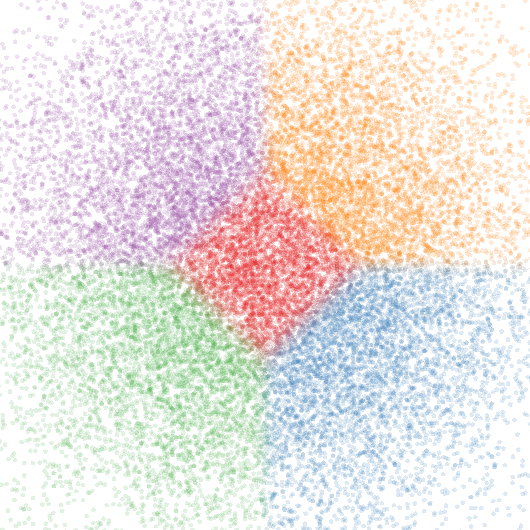
\includegraphics[width=0.3\columnwidth]{figures/deep_draws/deep_gp_sample_layer_1} &
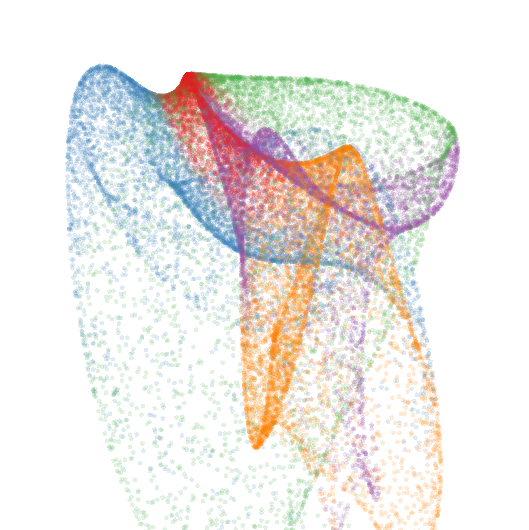
\includegraphics[width=0.3\columnwidth]{figures/deep_draws_connected/deep_sample_connected_layer2} &
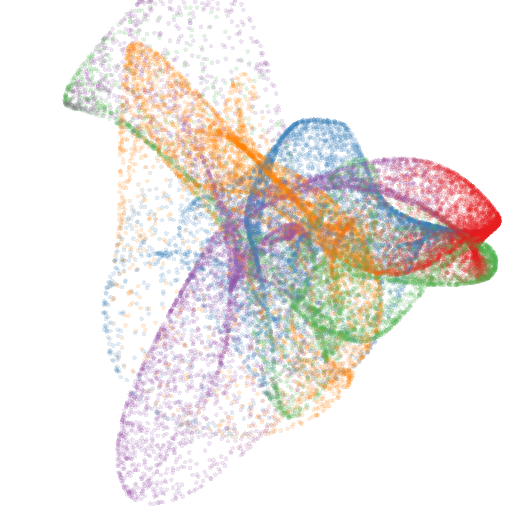
\includegraphics[width=0.3\columnwidth]{figures/deep_draws_connected/deep_sample_connected_layer3} \\
$p(\vx)$ & $p(f_1(\vx))$ & $p(f_2(f_1(\vx), \vx))$ \\ \\
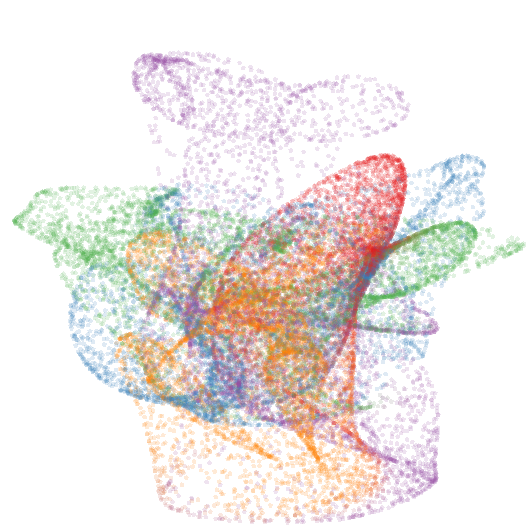
\includegraphics[width=0.3\columnwidth]{figures/deep_draws_connected/deep_sample_connected_layer4} &
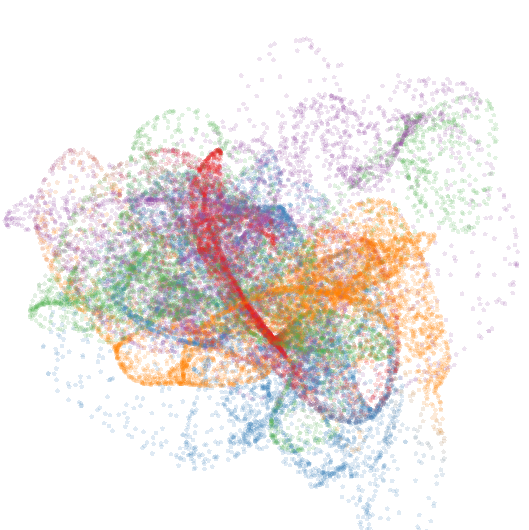
\includegraphics[width=0.3\columnwidth]{figures/deep_draws_connected/deep_sample_connected_layer5} &
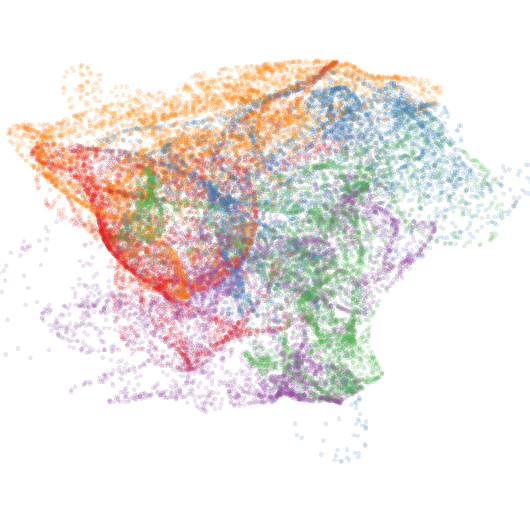
\includegraphics[width=0.3\columnwidth]{figures/deep_draws_connected/deep_sample_connected_layer6} \\
$p(f_3(f_2(f_1(\vx),\vx),\vx))$ & $p(f_4(f_3(f_2(f_1(\vx), \vx),\vx),\vx))$ & $p(f_5(f_4(f_3(f_2(f_1(\vx),\vx),\vx),\vx),\vx))$
\end{tabular}
\caption{Draws from a deep GP, with each layer connected to the input $\vx$.  By always depending on the original input, the density becomes more complex without concentrating along filaments.}
\label{fig:no_filamentation}
\end{figure}
%
%
%
%
\newcommand{\mappiccon}[1]{\includegraphics[width=0.3\columnwidth]{figures/map_connected/latent_coord_map_layer_#1}}
%
\begin{figure}
\centering
\begin{tabular}{ccc}
\mappic{0} & \mappiccon{1} & \mappiccon{2} \\
Identity Map: $\vy = \vx$ & 1 Layer: $\vy = f_1(\vx)$ & 2 Layers: $\vy = f_1(f_2(\vx), \vx)$ \\
\mappic{4} & \mappiccon{10} & \mappiccon{40} \\
4 Layers & 10 Layers & 40 Layers
\end{tabular}
\caption{Feature Mapping of a deep GP with each layer connected to the input $\vx$.  Just as the densities in \ref{fig:no_filamentation} became remain locally two-dimensional even after many transformations, in this mapping there are locally usually two directions that one can move $\vx$ in to change $\vy$.}
\label{fig:deep_map_connected}
\end{figure}






\section{Arbitarily Deep Kernels}
\label{sec:deep_kernels}

These types of kernels were originally investigated by \cite{cho2012kernel}.  In this section, we take the infinite limits of these compositions, and propose a new variant.



One can derive a Gaussian process as a neural network: $f(x) = {\mathbf \alpha}^T \Phi(x) = \sum_{i=i}^K \alpha_i \phi_i(x)$.  We can consider applying the feature transform $\Phi(\cdot)$ to the features themselves:  $\Phi_2 = \Phi(\Phi(\vx))$, 

In this section, we derive a kernel which corresponds to arbitrarily many compositions of the feature vectors corresponding to the squared-exp kernel:
%
\begin{align}
%k_1(\vx, \vx') & = \exp \left( -\frac{1}{2} ||\vx - \vx'||_2^2 \right) \\
k_2(\vx, \vx') & = \exp \left( -\frac{1}{2} || \Phi(\vx) - \Phi(\vx')||_2^2 \right) \\
k_2(\vx, \vx') & = \exp \left( -\frac{1}{2} \sum_i \left[ \phi_i(\vx) - \phi_i(\vx') \right]^2 \right) \\
k_2(\vx, \vx') & = \exp\left ( -\frac{1}{2} \sum_i \left[ \phi_i(\vx)^2 - 2 \phi_i(\vx) \phi_i(\vx') + \phi_i(\vx')^2 \right] \right) \\
k_2(\vx, \vx') & = \exp \left( -\frac{1}{2} \left[ \sum_i \phi_i(\vx)^2 - 2 \sum_i \phi_i(\vx) \phi_i(\vx') + \sum_i \phi_i(\vx')^2 \right] \right) \\
k_2(\vx, \vx') & = \exp \left( -\frac{1}{2} \left[ k_1(\vx, \vx) - 2 k_1(\vx, \vx') + k_1(\vx', \vx') \right] \right) \\
k_2(\vx, \vx') & = \exp \left( k_1(\vx, \vx') - 1 \right)
\end{align}
%
\begin{figure}
\centering
\begin{tabular}{ccc}
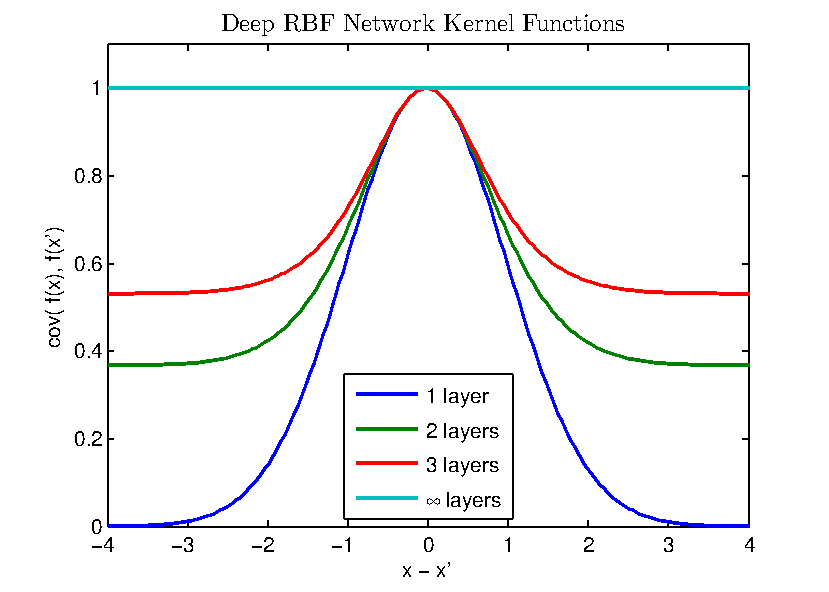
\includegraphics[width=0.5\columnwidth, clip, trim = 0cm 0cm 0cm 0.61cm]{figures/deep_kernel} &
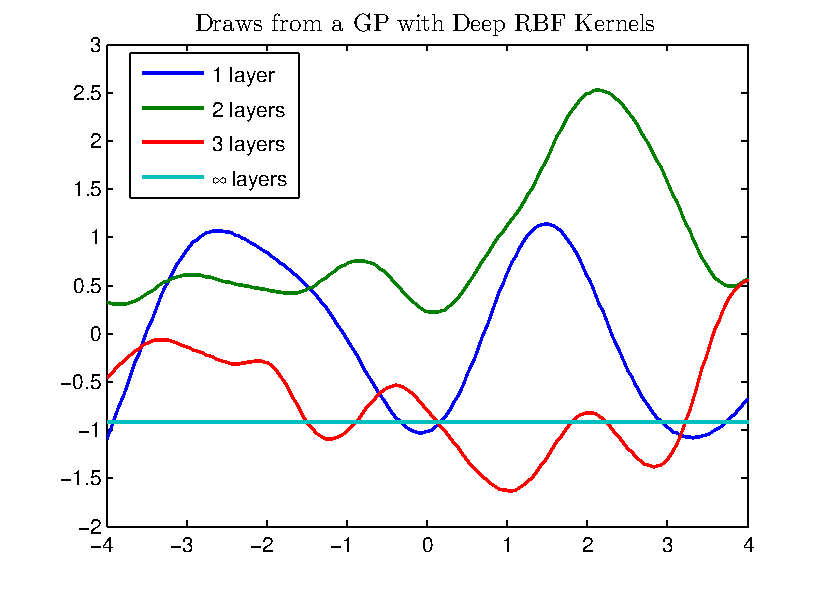
\includegraphics[width=0.5\columnwidth, clip, trim = 0cm 0cm 0cm 0.61cm]{figures/deep_kernel_draws} \\
Kernel derived from iterated feature transforms & Draws from the corresponding kernel
\end{tabular}
\caption{A degenerate kernel produced by repeatedly applying a feature transform.}
\label{fig:deep_kernel}
\end{figure}
%
Thus if $k_1(x,y) = e^{-||x - y||2}$, then the two-layer kernel is simply $k_2(x,y) = e^{k_1(x, y) - 1}$.  This formula is true for every layer: $k_{n+1}(x,y) = e^{k_n(x, y) - 1}$.
%
Note that nothing in this derivation depends on details of $k_1$, except that $k_1( \vx, \vx) = 1$.  Because this is true for $k_2$ as well, this recursion holds in general, and we have that $k_{n+1}(x,y) = e^{k_n(x, y) - 1}$.  In the infinite limit, this recursion converges to $k(x,y) = 1$ for all inputs.

Figure \ref{fig:deep_kernel} shows this kernel at different depths, including the degenerate limit.  One interpretation of why repeated feature transforms lead to this degenerate prior is that each layer can only lose information about the previous set of features.  In the limit, the transformed features contain no information about the original input $\vx$.  Since the function doesn't depend on its input, it must be the same everywhere.



\subsection{Fixing the deep kernel}

Follow a suggestion from Radford Neal's thesis \cite{neal1995bayesian}, we connect the inputs to each layer of features.  We do this simply by augmenting the feature vector $\Phi_n(\vx)$ with the extra features $\vx$ at every layer:
%
\begin{align}
%k_1(\vx, \vx') & = \exp \left( -\frac{1}{2} ||\vx - \vx'||_2^2 \right) \\
k_{n+1}(\vx, \vx') & = \exp \left( -\frac{1}{2} \left|\left| \left[ \! \begin{array}{c} \Phi_n(\vx) \\ \vx \end{array} \! \right]  - \left[ \! \begin{array}{c} \Phi_n(\vx') \\ \vx' \end{array} \! \right] \right| \right|_2^2 \right) \\
k_{n+1}(\vx, \vx') & = \exp \left( -\frac{1}{2} \sum_i \left[ \phi_i(\vx) - \phi_i(\vx') \right]^2 -\frac{1}{2} || \vx - \vx' ||_2^2 \right) \\
%k_{n+1}(\vx, \vx') & = \exp\left ( -\frac{1}{2} \sum_i \left[ \phi_i(\vx)^2 - 2 \phi_i(\vx) \phi_i(\vx') + \phi_i(\vx')^2 \right]  -\frac{1}{2} || \vx - \vx' ||_2^2 \right) \\
%k_2(\vx, \vx') & = \exp \left( -\frac{1}{2} \left[ \sum_i \phi_i(\vx)^2 - 2 \sum_i \phi_i(\vx) \phi_i(\vx') + \sum_i \phi_i(\vx')^2 \right] \right) \\
%k_2(\vx, \vx') & = \exp \left( -\frac{1}{2} \left[ k_1(\vx, \vx) - 2 k_1(\vx, \vx') + k_1(\vx', \vx') \right] \right) \\
k_{n+1}(\vx, \vx') & = \exp \left( k_1(\vx, \vx') - 1 -\frac{1}{2} || \vx - \vx' ||_2^2 \right)
\end{align}
%
Thus, this kernel satisfies the recurrence $k - \log(k) = 1 + \frac{1}{2} || \vx - \vx' ||_2^2$.  

\paragraph{Properties of this kernel} The solution to this recurrence has no closed form, but it is continuous and differentiable everywhere except at $\vx = \vx'$.

Conjectures:  
\begin{itemize}
\item Samples from a GP with this prior are not differentiable.
\item This kernel has smaller covariance than the squared-exp everywhere except at $\vx = \vx'$.  
\item Samples from this kernel are fractal.
\end{itemize}


\begin{figure}
\centering
\begin{tabular}{ccc}
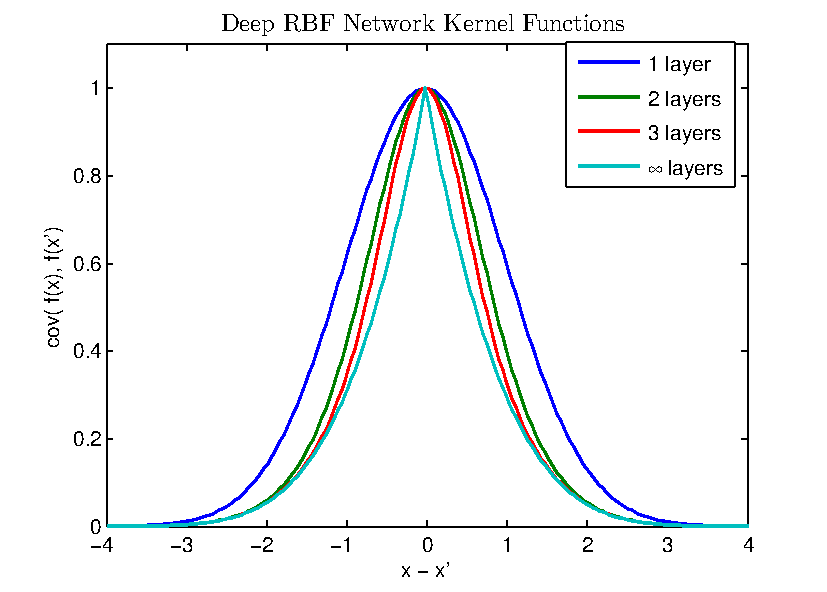
\includegraphics[width=0.5\columnwidth, clip, trim = 0cm 0cm 0cm 0.61cm]{figures/deep_kernel_connected} &
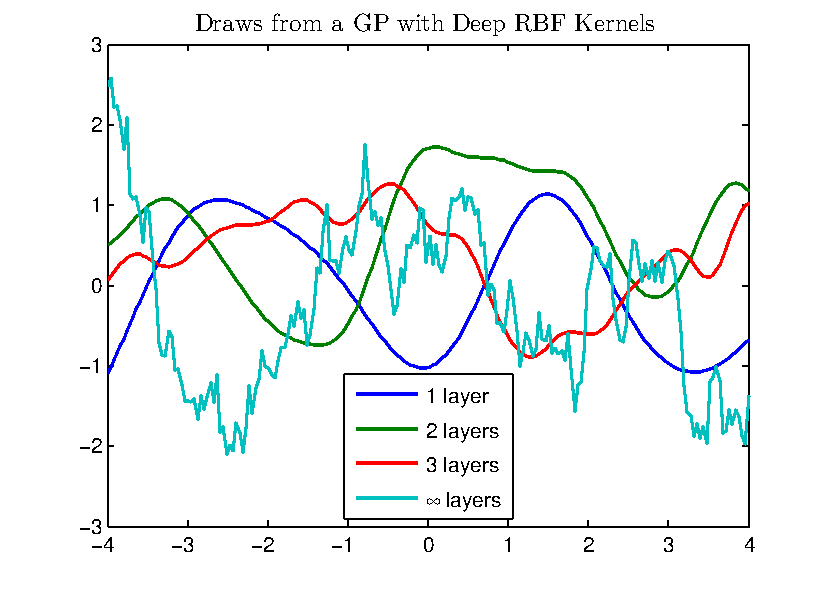
\includegraphics[width=0.5\columnwidth, clip, trim = 0cm 0cm 0cm 0.61cm]{figures/deep_kernel_connected_draws} \\
Kernel derived from iterated feature transforms & Draws from the corresponding kernel \\
with all layers connected to the input &
\end{tabular}
\caption{A non-degenerate version of the infinitely deep feature transform kernel.  By connecting the inputs $\vx$ to each layer, the function can still depend on its input even after arbitrarily many layers of computation.}
\label{fig:deep_kernel_connected}
\end{figure}


\section{Related Work}

\subsection{A Survey of deep architectures}

\paragraph{Deep Density Networks}

\paragraph{Bayesian Deep Networks} \cite{adams2010learning} developed a prior on finite but unboundedly deep neural networks, each layer having a finite but unbounded number of hidden units.
\paragraph{Sum-product networks} introducted by \cite{poon2011sum}.

\paragraph{Feature Composition Kernels} \cite{cho2012kernel} developed kernels of the type discussed in section \ref{sec:deep_kernels}, and investigated them experimentally.

\paragraph{Recurrent Neural Networks}

\paragraph{Dynamical Systems}

These architectures are all constructed in a stacked manner, with connections only between adjacent layers.


[Warping a 1d uniform distribution]


\subsection{Related Analyses}

\cite{montavon2010layer} note that performance of a MLP degrades as the number of layers with random weights increases.
%\url{http://books.nips.cc/papers/files/nips23/NIPS2010_0206.pdf}


\section{Conclusions}

\paragraph{Deep neural networks and deep Gaussian processes are analyzable using random matrix theory.}  After proving that the Jacobian is an i.i.d. Gaussian matrix, many other forms of 

\paragraph{If you want to use very deep nets, you won't be able to do so if you initialize/regularize all your weights independently}  We might want to think about different ways of 

\paragraph{If you initialize independently, the density becomes fractal} Points close in $x$-space can be very far in $y$-space, and vice versa.

\paragraph{A spikey eigenspecturm will lead to saturation}
Maybe we should initialize differently in order to avoid such saturation, like Martens' sparse initialization: \url{http://www.cs.toronto.edu/~jmartens/docs/Deep_HessianFree.pdf}




\subsubsection*{Acknowledgments}

We would like to thank Andrew McHutchon, Neil Lawrence, Josh Tenenbaum, Andreas Diamanadou, James Lloyd, and Mark van der Wilk for helpful discussions.

\bibliographystyle{plainnat}
\bibliography{verydeep}


\end{document}























\paragraph{Approach}
We are going to analyze these networks by looking at the neighbourhood surrounding random points.

\subsection{Different settings}

In our analysis, we assume that functions are normalized.



\begin{itemize}
\item The kernel is an RBF, meaning that all functions are infinitely differentiable.  This also corresponds to the infinite limit taken by Radford Neal [cite]
\item The dimension of the latent space is always the same.
\end{itemize}

We consider several different variations of deep GPs:

\begin{itemize}
\item mean function $m_d(x_d) = 0$
\item mean function $m_d(x_d) = x_d$
\end{itemize}

\paragraph{Noise versus no noise}
Do the deep functions we're interested in modeling have noise added at each step?  Consider the example of handwritten digits.  One putative model would be that $x$ is the number that the human is trying to write, then a series of functions of his nervous system and arm (with feedback loops) cascade to produce the observed digit.  This whole process can be expected to have small amounts of noise at each step, but presumably \emph{can only work if the amount of noise is small}.

A function whose result gets a lot of noise added at each intermediate step is probably not useful unless there is an error-correcting step applied downstream.  Perhaps our results hold because random functions do not do error-correction.  Perhaps this is another intuition for why 'dropout' works - functions are explicitly trained to be robust to noise.  Denoising autoencoders are also trained in this way.

\begin{itemize}
\item Density models
\item Function models
\end{itemize}




\begin{align}
\textrm{Filament}(p(\vx)) = 1 - \int \frac{ \bar \lambda}{ \lambda_\textrm{min}} p(\vx) d\vx
\end{align}

where $\lambda_\textrm{min}$ is the smallest eigenvalue of the Hessian of $p(\vx)$.

There is some sort of connection between average eigenvalue and signal power:
[\url{http://www1.i2r.a-star.edu.sg/~yhzeng/ZENG-TCOM-09-0402.pdf}]

This definition doesn't depend on scale, although it does depend on parameterization in general.

\paragraph{Example: A uniform distribution of any dimension}
A uniform distribution has $\textrm{Filament}(p(\vx)) = 0$.

\paragraph{Example: Any distribution defined over 1 dimension}
In one dimension, there is only one eigenvalue, so $ \bar \lambda = \lambda_\textrm{min}$, and thus $\frac{ \bar \lambda}{ \lambda_\textrm{min}} = 1$ everywhere.  So every 1D distribution has $\textrm{Filament}(p(\vx)) = 0$.

\paragraph{Example: A 1D sigmoid in two dimensions}
A 1d sigmoidal-shaped distribution in two dimensions will have $\textrm{Filament}(p(\vx)) > 0$, because at the top of the curve, $\frac{ \bar \lambda}{ \lambda_\textrm{min}} > 1$, and this can't be cancelled out, because everywhere else, $\frac{ \bar \lambda}{ \lambda_\textrm{min}} \geq 1$.

\subsection{Why does filamentation occur?}
Intuition: The space will be squished in some directions, and stretched in others.  However, any direction's Jacobian will be a product of lots of directional Jacobians.  This distribution will become heavy-tailed, meaning that it will be dominated by a few small values.  We can characterize the ratio of the maximum direction of curvature to the average.




\paragraph{The Hessian of a deep density model}

Since we know the density of a point drawn from a deep GP, we can also look at the local curvature through the Hessian.  Given an $\vx, \vy$ pair $\vy = f(\vx)$, 
%
\begin{align}
p(\vy) 
= \frac{p_x( f\inv(\vy ))}{\left| J( f\inv(\vy)) \right|} 
= \frac{p_x( \vx )}{\left| J( \vx) \right|}
= p_x( \vx ) \left| J( \vx)\inv \right|
\end{align}
%
So we can say that the determinant of the inverse transform $\left| J( \vx)\inv \right|$ defines the local distortion of density.

We want to know how many directions we can move in.

We could characterize this by the probability, if we moved in a random direction, of not moving into a region of low probability.  If we're at a local maximum, we can ask how many eigenvalues of the Hessian are small.


The Hessian of the determinant of the Jacobian is:
\begin{align}
H_y \left( \left| J_{\vy \rightarrow \vx} (\vy) \right| \right)
 & = \begin{bmatrix}
\dfrac{\partial^2 \detJyy}{\partial y_1^2} & \dfrac{\partial^2 \detJyy}{\partial y_1\,\partial y_2} & \cdots & \dfrac{\partial^2 \Jyy}{\partial y_1\,\partial y_n} \\[2.2ex]
\dfrac{\partial^2 \detJyy}{\partial y_2\,\partial y_1} & \dfrac{\partial^2 \detJyy}{\partial y_2^2} & \cdots & \dfrac{\partial^2 \detJyy}{\partial y_2\,\partial y_n} \\[2.2ex]
\vdots & \vdots & \ddots & \vdots \\[2.2ex]
\dfrac{\partial^2 \detJyy}{\partial y_n\,\partial y_1} & \dfrac{\partial^2 \detJyy}{\partial y_n\,\partial y_2} & \cdots & \dfrac{\partial^2 \detJyy}{\partial y_n^2}
\end{bmatrix} \\
 & = H_y \left( \left| \Jyy \right| \right) \\
 & = H_y \left( \prod_i \lambda^{\Jy}_i ( \vy) \right) \qquad \textrm{where $\lambda$ are eigenvalues of $\Jyy$}
 \\
 & = H_y \left( \prod_i \frac{1}{\lambda^{\Jx}_i ( \vx )} \right)
\end{align}
%
where $H_y$ means that the second derivatives in the Hessian are taken w.r.t. $\vy$, and $\lambda^{J\inv}_i ( \vx)$ are the eigenvalues of the Jacobian (the total derivative of $f\inv(\vy)$ w.r.t. $\vx$).

\paragraph{Derivative of determinant}
\begin{align}
\frac{\partial \det(A)}{\partial A_{ij}}= \operatorname{adj}(A)_{ji}= \det(A)(A^{-1}_{ji}) \\
\frac{\mathrm{d} \det(A)}{\mathrm{d} \alpha} =  \det(A) \operatorname{tr}\left(A^{-1} \frac{\mathrm{d} A}{\mathrm{d} \alpha}\right)
\end{align}
%
In our case, we have:
%
\begin{align}
\frac{\partial \det(\Jyy)}{\partial \vy_i} & = \det(\Jy) \trace \left(\Jx \frac{\partial \Jyy}{\partial \vy_i}\right) \\
& = \det(\Jy) \trace \left( - \Jx \Jy \frac{\partial \Jx(\vy)}{\partial \vy_i} \Jy \right) \\
& = \det(\Jy) \trace \left( - \frac{\partial \Jx(\vy)}{\partial \vy_i} \Jy \right) \\
& = \det(\Jy) \trace \left( - \frac{\partial \Jx(\vx)}{\partial \vx} \frac{\partial \vx}{\partial \vy_i} \Jy \right) \\
& = \det(\Jy) \trace \left( - \frac{\partial \Jx(\vx)}{\partial \vx} \Jy^{:,i} \Jy \right) \\
& = \det(\Jy) \trace \left( - \Jy \frac{\partial \Jx(\vx)}{\partial \vx} \Jy^{:,i} \right) \label{eqn:ddet_tractable} \\
& = \det(\Jy) \trace \left( \frac{\partial \Jy(\vy)}{\partial \vx} \right)
\label{eqn:ddet_simple}
\end{align}
%
We don't have an analytic form for \eqref{eqn:ddet_simple}, but we can compute \eqref{eqn:ddet_tractable} if we can compute the term $\frac{\partial \Jx(\vx)}{\partial \vx}$, which is just the second derivative of $\fdeep(\vx)$.

\paragraph{Derivative of SVD}
a

\url{http://www.ics.forth.gr/_publications/2000_eccv_SVD_jacobian.pdf} says that:
%
\begin{align}
\frac{\partial \det(A)}{\partial A_{ij}}= \operatorname{adj}(A)_{ji}= \det(A)(A^{-1}_{ji})
\end{align}



\paragraph{Hessian of determinant}
\begin{align}
\frac{\partial^2 \det(A)}{\partial A_{ij}\partial A_{mn}}
& = \det(A)(A^{-1}_{ji}A^{-1}_{nm} - A^{-1}_{ni}A^{-1}_{jm})
\end{align}

We can also say that

\url{http://math.stackexchange.com/questions/50386/the-hessian-of-the-determinant}

\begin{align}
\frac{\partial^2 \det(A(\vy))}{\partial y_i \partial y_j}
& = \frac{\partial^2 \det(A(\vy))}{\partial A_{ij}\partial A_{mn}} \left( \frac{\partial A_{ij}}{\partial y_i} + \frac{\partial A_{ij}}{\partial y_j} \right) \left( \frac{\partial A_{mn}}{\partial y_i} + \frac{\partial A_{mn}}{\partial y_j} \right)
%& = \det(A)(A^{-1}_{ji}A^{-1}_{nm} - A^{-1}_{ni}A^{-1}_{jm})
\end{align}

or we can try:

\begin{align}
\frac{\partial^2 \det(A(\vy))}{\partial y_i \partial y_j}
& = \frac{\partial }{\partial \vy_j} \det(\Jy) \trace \left( \frac{\partial \Jy(\vy)}{\partial \vx} \right) \\
& = \det(\Jy) \frac{\partial }{\partial \vy_j} \trace \left( \frac{\partial \Jy(\vy)}{\partial \vx} \right) 
  + \trace \left( \frac{\partial \Jy(\vy)}{\partial \vx} \right) \frac{\partial }{\partial \vy_j} \det(\Jy) \\
\end{align}

or:

\begin{align}
\frac{\partial^2 \det(A(\vy))}{\partial y_i \partial y_j}
= \det(A) & \Big[ 
          \trace \left( A\inv \frac{\partial^2 A(\vy)}{\partial \vy_i \partial \vy_j } \right) \nonumber \\
          & + \trace \left( A\inv \frac{\partial A(\vy)}{\partial \vy_i} \right) 
            \trace \left( A\inv \frac{\partial A(\vy)}{\partial \vy_j} \right) \nonumber \\
           & + \trace \left( A\inv \frac{\partial A(\vy)}{\partial \vy_i} 
                          A\inv \frac{\partial A(\vy)}{\partial \vy_j} \right)
         \Big] \\
\frac{\partial^2 \det(\Jy(\vy))}{\partial y_i \partial y_j}
= \det(\Jy) & \Big[
          \trace \left( \Jy\inv \frac{\partial^2 \Jy(\vy)}{\partial \vy_i \partial \vy_j } \right) \nonumber \\
          & + \trace \left( \Jy\inv \frac{\partial \Jy(\vy)}{\partial \vy_i} \right) 
            \trace \left( \Jy\inv \frac{\partial \Jy(\vy)}{\partial \vy_j} \right) \nonumber \\
           & + \trace \left( \Jy\inv \frac{\partial \Jy(\vy)}{\partial \vy_i} 
                          \Jy\inv \frac{\partial \Jy(\vy)}{\partial \vy_j} \right)
         \Big] \\
= \det(\Jy) & \Big[
          \trace \left( \Jx \frac{\partial^2 \Jy(\vy)}{\partial \vy_i \partial \vy_j } \right) \nonumber \\
          & + \trace \left( \Jx \frac{\partial \Jy(\vy)}{\partial \vy_i} \right) 
            \trace \left( \Jx \frac{\partial \Jy(\vy)}{\partial \vy_j} \right) \nonumber \\
           & + \trace \left( \Jx \frac{\partial \Jy(\vy)}{\partial \vy_i} 
                          \Jx \frac{\partial \Jy(\vy)}{\partial \vy_j} \right)
         \Big] \\        
%
%\frac{\partial^2 \det(A(\vy))}{\partial A_{ij}\partial A_{mn}} \left( \frac{\partial A_{ij}}{\partial y_i} + \frac{\partial A_{ij}}{\partial y_j} \right) \left( \frac{\partial A_{mn}}{\partial y_i} + \frac{\partial A_{mn}}{\partial y_j} \right)
%& = \det(A)(A^{-1}_{ji}A^{-1}_{nm} - A^{-1}_{ni}A^{-1}_{jm})
\end{align}

\paragraph{Eigenvalues of Hessian}





\section{Random Matrix Theory}

``On the number of real eigenvalues of products of random matrices and an application to quantum entanglement''
\url{http://arxiv.org/pdf/1301.7601v1.pdf}

\paragraph{Stationarity} When characterizing deep \gp{}s, having a stationary kernel means that expectations of our function will be the same no matter which point we evaluate it at.  In other words, for any statistic $S(f(\vx))$, $\expect [ S( f(\vx) ] = \expect [ S( f(\vx') ] \forall \vx \forall \vx'$.  
%This is not true in general for deep \gplvm{}s.




%\begin{proposition}
\paragraph{The mean of a deep zero-mean \gp{} has mean zero.}
%The mean of a deep zero-mean \gp{} has mean zero.
%\end{proposition}
%
%\begin{proof}[Proof]
All functions are drawn \iid, so we can ignore all but the last transformation $f_L$.  Since $f_L$ is zero-mean, then $\forall \vx \forall d, \expectargs{\GP}{f_d(x)} = 0 $.
%\end{proof}


\subsection{Properties of the Jacobian}

\subsection{Gaussian Processes}

\subsection{Gaussian Process Latent Variable Model}

\begin{figure}
\centering
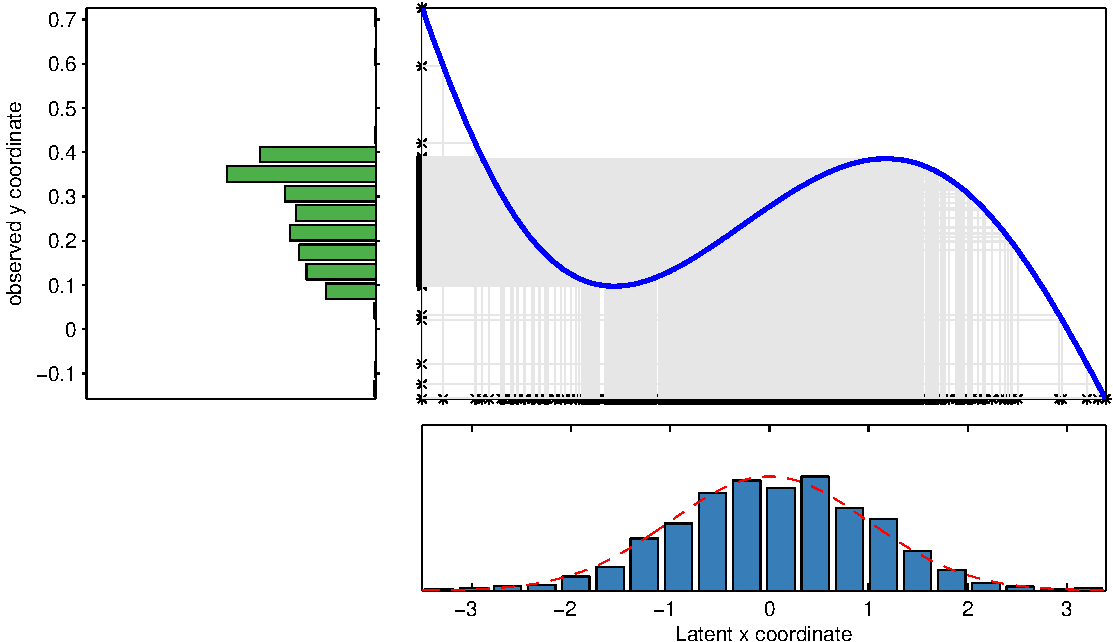
\includegraphics[width=0.8\columnwidth]{figures/gplvm_1d_draw_8} 
\caption{A draw from a Gaussian process latent variable model.  Bottom:  The latent datapoints $\vX$ are distributed according to a parametric base distribution (a Gaussian).  Top right:  A smooth function $f$ drawn from a Gaussian process prior is applied to obtain $\vY$ = $f(\vX)$.  Left:  The observed data $\vY$ is distributed according to a non-Gaussian density.}
\label{fig:gplvm_intro}
\end{figure}

The GP-LVM specifies a model wherein latent variables $\vX$ are warped by an unknown smooth, function $f$ to produce the observed data $\vY$.  The prior used over functions in the GP-LVM is the Gaussian process~\cite{rasmussen38gaussian}.

While not typically thought of as a density model, the GPLVM does define a nonparametric density over observations~\cite{nickisch2010gaussian}.   Figure \ref{fig:gplvm_intro} demonstrates how a Gaussian latent density, when warped by a random smooth function, can give rise to a non-Gaussian density in the observed space.

The dimension of the observed data ($D$) doesn't need to match the dimension of the latent space ($Q$).  When $Q$ is 2 or 3, the GP-LVM can also be used for visualization of high-dimensional data.  The mapping from $\vX$ to each dimension of the observed data is assumed to be independent, so the likelihood has a simple form which implicitly integrates over $f$:
%
\begin{align}
p(\vY | \vX,\bm{\theta})  = (2 \pi)^{-\frac{DN}{2}}  |\vK|^{-\frac{D}{2}} \exp \left( -\frac{1}{2} {\rm tr}( \vY^{\top} \vK^{-1} \vY) \right),
\label{eq:py_x}
\end{align}
where $\vK$ is the $N \times N$ covariance matrix defined 
by the kernel function $k(\vx_{n},\vx_{m})$,
and $\bm{\theta}$ is the kernel hyperparameter vector.
In this paper, we use an RBF kernel with an additive noise term:
\begin{align}
k(\vx_{n},\vx_{m}) &= \alpha \exp\left( - \frac{1}{2 \ell^2}(\vx_n - \vx_m)^{\top} (\vx_n - \vx_m) \right) + \delta_{nm} \beta^{-1}.
\end{align}




\paragraph{The density in the observed space of a deep density}

Let $\vy = \fdeep(\vx)$ be a random variable.
%
The change-of-variables formula is:
\begin{align}
p(f(\vx)) = \sum_{k=1}^{n(\vy_k = f(\vx_k))} \left| \frac{d}{dy} f^{-1}(\vy_{k}) \right| \cdot p_x(\vx_{k})
\end{align}
%
Assuming that $\fdeep(\vx)$ is one-to-one,
\begin{align}
p(f(\vx)) = p_x( \vx ) \left| \frac{  \partial f\inv(x) }{\partial x } \right|
\end{align}
%
We can use that
\begin{align}
\det(A\inv) = \frac{1}{\det(A)}
\end{align}
%
Assuming that $\fdeep(\vx)$ is one-to-one,
\begin{align}
p(f(\vx)) = p_x( \vx ) \left| J\inv(\vx) \right| = p_x( \vx ) \frac{1}{\left| J(\vx) \right|}
\end{align}

\paragraph{Eigenvalues of inverse}  We can try to prove things about the eigenvalues of $J(\vx)$.  However, in order to characterize the density of $p(\vy)$, we will need to analyse the eigenspectrum of $J\inv(\vx)$.  Helpfully, if $\lambda$ are the eigenvalues of $J$, then $\lambda \inv$ are the eigenvalues of $J\inv$.

\paragraph{Determinant in terms of Eigenvalues}  If $\lambda$ are the eigenvalues of J, then
\begin{align}
|J| = \prod_i \lambda_i
\end{align}







\section{Relation to Deep Neural Networks}

There are two reasons to think that the deep-GP prior is related to the inductive bias of deep neural networks.  First, the 

\paragraph{Weights don't change much during training}
James Martens says that the weights don't change much during training.  Perhaps we could make a plot showing the original weights versus the trained weights?

\paragraph{$L_2$ regularization of weights corresponds in a loose sense to independent Gaussian priors on the weights}
Which correspond to Gaussian processes (Neal)

